\chapter{Literature Review}\label{ch:literature-review}
\initial{T}his chapter will start a general overview of work and literature relevant to indoor positioning systems.
It will contain a critical analysis of existing technologies and address their advantages and disadvantages.
Additionally, the concept of sensor fusion will be summarised and its potential in localisation systems.
Finally, a section will be dedicated to cover work done with a commercial Ultra-Wide Band system known as Pozyx which much of this research revolved around.
\section{Indoor Localisation Systems}\label{sec:indoor-localisation-sensors}
\subsection{Passive Systems}\label{subsec:passive-systems}
%TODO: PUT IN MORE PAPERS CITING UWB AND WORK WITH UWB/POZYX -> look at the pozyx site
In summary, passive systems do not require the object being tracked to have some of the electronics on them to do positioning.
Some examples of passive systems are ~\citep{deak2012survey}:
\begin{itemize}
    \item Computer Vision and Imaging systems.
    \item Tactile and contact sensors.
    \item Attenuation of signals.
    \item Differential air pressure.
\end{itemize}
A common example of computer vision-based localisation is to use a setup consisting of multiple cameras in a space trying to detecting a single object.
Using the intrinsic and extrinsic properties of each camera it is possible to determine the transform to the object in a given frame with relatively high accuracy.
A prime example of this is the commercial VICON motion capture systems.
~\cite{aerialrobotsiitk} shows a drone application in which the UAV is positioned using a VICON motion capture system.
Figure~\ref{fig:vs} shows the simplified setup.
It should be noted that the UAV must be equipped with a specialised marker that is used to identify it.
Furthermore, the positions are fed to a companion computer connected to the autopilot system.
The VICON setup provides highly accurate positions and is often used to gather ground truth positional data to compare to other positioning systems.
The additional requirements of the VICON systems, however, do not make it feasible for indoor applications.

\begin{figure}[h!]
    \centering
    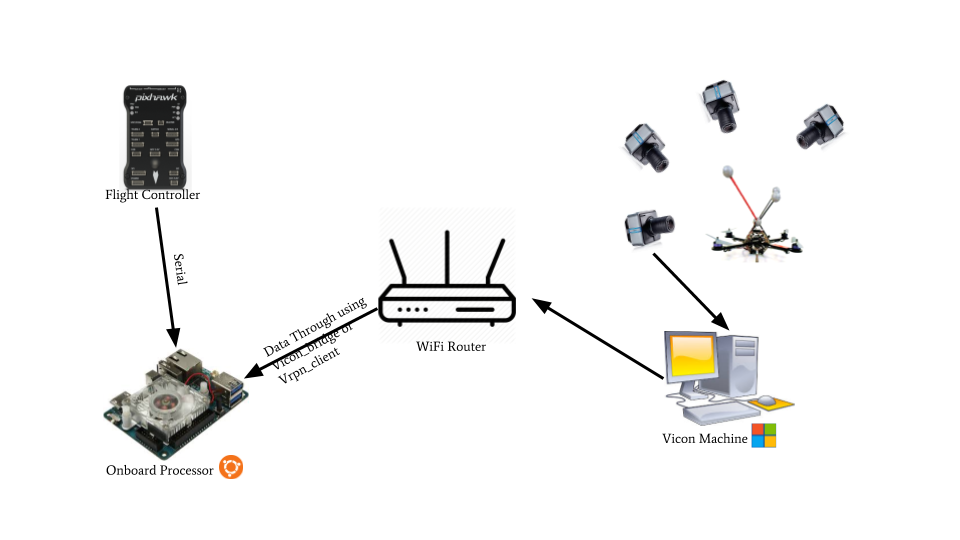
\includegraphics[scale=.45]{vicon_setup}
    \caption{VISON setup for position of a UAV. (\url{https://aerial-robotics-iitk.gitbook.io/wiki/estimation/setup-with-vicon})}
    \label{fig:vs}
\end{figure}

\subsection{Active Systems}
In contrast to passive systems, active systems have the object being positioned equipped with electronics.
Many indoor localisation techniques use this and some examples are ~\citep{deak2012survey}
\begin{itemize}
    \item Radio-frequency identification
    \item UWB
    \item Wireless Local Area Network
    \item Bluetooth Low Energy (BLE)
\end{itemize}
Many of these setups use an anchor and tag configuration.
The tag receives signals from multiple anchors and triangulates the tag.

An approach using and comparing UWB and BLE was developed by ~\cite{findobjs} to do localisation in a museum.
Both methods are combined with a dead reckoning system to improve accuracy.
Six paintings are equipped with both a BLE and UWB tag.
The test setup first did a calibration where both sensors were placed at fixed points in the museum with a clear line of sight to each tag.
From initial ranging performance, the UWB setup was shown to perform better with a distance variance of $\pm0.4m$ while the BLE setup had errors of over $10m$.
It is noted by the authors that a ranging approach with BLE is challenging since it uses an RSSI method but can match the accuracy of the UWB setup when combined with a dead reckoning system after some initial steps by the user.

\begin{figure}[h!]
    \centering
    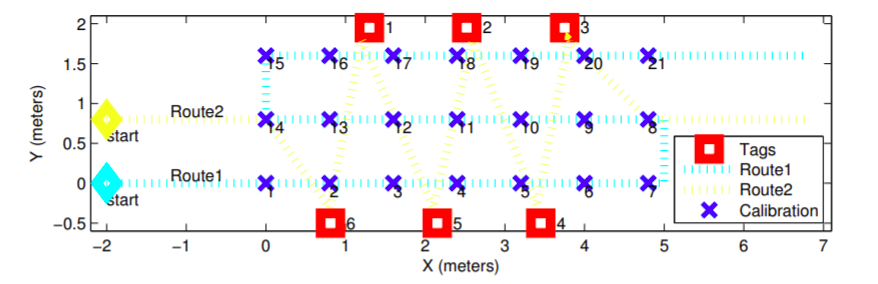
\includegraphics[scale=.45]{uwb_vs_ble}
    \caption{Setup used to compare UWB and BLE performance in a museum. \cite{findobjs} Page: 3}
    \label{fig:uwbvsble}
\end{figure}

\section{Sensor Fusion}\label{sec:sensor_fusion}
Appendix~\ref{app:app01} describes the basic operation of the Pozyx system which is based on Time of Flight (TOF) calculations.
With a tag it is possible to determine a rough estimate of the position in a given reference frame.
Additionally, the tag has an Inertial Measurement Unit (IMU), consisting of an Accelerometer, Gyroscope, Magnetometer and an Altimeter.
These are used in one of the operational modes of the Pozyx system in order to improve accuracy.
Sensor fusion combines multiple sources of data in order to get a fairly accurate estimate of the pose of the system,
The measurements from the tag can be combined with the sensors onboard an FCU in order to achieve this.
The de-facto sensor fusion technique is called the Extended Kalman Filter (EKF).
~\citet{simpleekf} documented a useful description and example of how the EKF works.
Algorithmically, the EKF is a recursive process using predictions based on the dynamics of the vehicles and updating the estimate based on these predictions and measurements from various sources.
The major requirement for the EKF is that the process model and the measurement model are differentiable.
The steps for the EKF are as follows:
\begin{enumerate}
    \item Provide and initial estimate for the state, $\hat{x}^+_k$, and the prediction error, $P^+_k$.
    \item Compute the Kalman gain, $K_k = P^+_{k}H_k^T(H_k P^+_{k}H_k^T + R)^{-1}$
    \item Update the estimate with measurement $z_k$, $\hat{x}_k=\hat{x}^+_k + K_k(z_k - h(\hat{x}^+_k))$
    \item Update the prediction error, $P_k = (I - K_k H_k)P^+_{k}$
    \item Project the state ahead, $\hat{x}^+_{k+1} = f(\hat{x}_k, u_k, w)$
    \item Project the Prediction error ahead, $P^+_{k+1} = A_k P_k A_k^T + Q_k$
    \item Start from Step 2 for the next time step.
\end{enumerate}
Where K represents the Kalman gain, R is the Measurement Noise Covariance Matrix, Q is the Process Noise Covariance matrix.
%TODO: Look at add in another sensor fusion for indoor navigation here-> Look at the online wiki i did lol
~\citet{tsai1998localization} documented work for localising a mobile robot using ultrasonic measurements.
Although, the system was a wheeled mobile robot instead of a UAV, the calculations using the TOF measurements and dead reckoning data as well as the use of an EKF to improve the pose estimates are similar to what is trying to be achieved in this current project.
A notable contribution of the work is the use of a voting scheme to obtain the best 'observation' for the robot's orientation before being fed into the EKF algorithm.


\section{Pozyx - Behind the Scenes}\label{sec:pozyx---behind-the-scenes}
This research project used a commercially available, active UWB sensor to aid in localisation of an indoor UAV system.
\begin{figure}[h!]
    \centering
    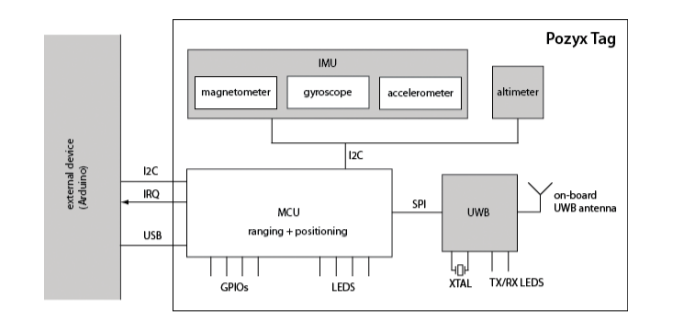
\includegraphics[scale=.7]{lr/uwb_block}
    \caption{Simplified Block Diagram of the Pozyx tag.}
%    \label{fig:twr}
\end{figure}
\subsection{Ultra-WideBand (UWB)}
The core of the Pozyx system operates using a UWB approach.
UWB is a short-range, low energy, high bandwidth communication radio technology.
Radio waves travel at the speed of light ($c=299792458ms^{-1}$) so using a TOF approach the range between a tag and an anchor can be obtained simply by:
\[
    d = c*TOF
\]

Knowing the position of each anchor in a given reference frame, ~\citet{evaluwb} discussed a method to use raw range readings in order to determine the position of the tag.
The positions can be described by the following system of equations:
        \begin{equation}
                \left[
            \begin{array}{c}
                (x - x_1)^2 + (y - y_1)^2 + (z - z_1)^2 = d_1^2\\
                \vdots\\
                (x - x_n)^2 + (y - y_n)^2 + (z - z_n)^2 = d_n^2
            \end{array}
                \right]
        \end{equation}
        Where $n$ represents an index of an anchor and $(x,y,z)$ represents the position of the tag.
        This was converted into matrix form of \textbf{A.x = B}:
        \begin{equation}
            \left[
            \begin{array}{c}
                1 - 2x_1 -2y_1 -2z_1\\
                \vdots\\
                1 - 2x_n -2y_n -2z_n
            \end{array}
            \right]
        *
            \left[
                \begin{array}{c}
                    x^2 + y^2 +z^2\\
                    x\\
                    y\\
                    z\\
                \end{array}
            \right]
            =
        \left[
            \begin{array}{c}
                d_1^2 - x_1^2 - y_1^2 -z_1^2\\
                \vdots\\
                d_n^2 - x_n^2 - y_n^2 -z_n^2
            \end{array}
        \right]
       \end{equation}

        The position of the tag can be calculated as:
        \[
            \hat{x} = (A^{T}A)^{-1}A^{T}B
        \]

From the algorithms and work presented we can confirm that the Pozyx system can achieve an accuracy of $\pm10cm$ in standard environments with LOS.
The work confirms that LOS of the anchors to tag is a major factor in accuracy and this will be taken into account when anchors are being placed in the research.
Furthermore, the work mentioned in this section proposes an algorithm with raw range readings in order to do localisation, my research will focus on the integration of the Pozyx tag with a standard FCU, so the pose data coming directly from the tag can be used.
The pose can be obtained via two modes: 1). A pure Two Way Ranging (TWR) Approach or 2.) A tracking approach using a Kalman prediction filter in addition to the TWR pose.
%TODO: MARK HERE WITH MORE PAPERS EXPANDING UWB

Additional work done by ~\citet{di2019evaluation} also performs an evaluation of UWB systems for indoor applications.
The work compares several commercial UWB systems available to consumers and their viability in ranging and pose estimation.
The sensors are treated as black-box systems and the proprietary algorithms for each system were used.
The results documented in this paper show useful steps for a primary evaluation of multiple anchor configurations in a given space.

\subsection{Pozyx Localisation}\label{subsec:pozyx-localisation}
In contrast to the raw readings obtained in the previous work, the Pozyx system has been used in several localisation systems, both indoors and outdoors.
Experiments done by ~\citet{destefano2019using} use the Pozyx system in multiple scenarios for the purpose of education.
The setup is simple and the two-dimensional positions, x and y, form the basis of  graphs that can be used to determine average velocities from linear interpolation of a position versus time graph.
Figures ~\ref{fig:bpozyx} and ~\ref{fig:stupozyx} show both how the physical setup looked and some of the data collected.
Although the UWB positioning system has advantages over several other systems the researchers note that using the Pozyx system in this scenario is not ideal for several reasons.
The accuracy of the system ($\pm10cm$) leads to large variance in instantaneous velocity when calculations are done on a point to point basis.

\begin{figure}[h!]
    \centering
    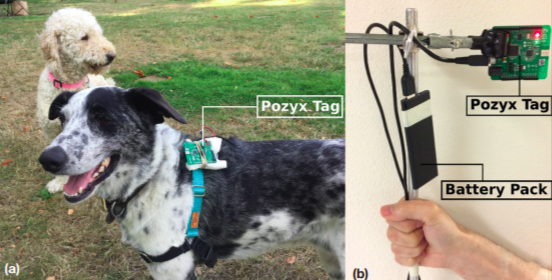
\includegraphics[scale=.5]{lr/bork_pozyx}
    \caption{The experimental setups for both a dog and a student. \cite{destefano2019using} Page: 1.}
    \label{fig:bpozyx}
\end{figure}

\begin{figure}[h!]
    \centering
    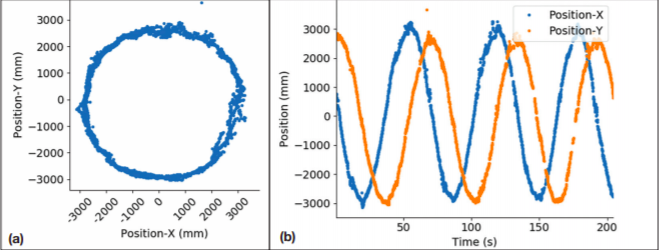
\includegraphics[scale=.5]{lr/student_walking_results}
    \caption{Data collected from a student walking in a circle. \cite{destefano2019using} Page: 2.}
    \label{fig:stupozyx}
\end{figure}

~\citet{conceiccao2017robot} present a method for using the Pozyx in an outdoor environment.
The systems operated in two ways: 1.) Using raw range values from the Pozyx sensor and using an EKF externally for pose estimates. 2.) The pose estimates coming from the Pozyx sensor itself.
A modified version of the EKF is described in the first scenario.
An additional check is done for outliers.
Outliers can be described as measurements that do not fit the pattern of the previous measurements.
If an outlier is detected it is simply not considered in that time step and the previously calculated values are used instead.
The test environment was an outdoor scenario with a range error characterisation test which allowed for optimal anchor placement and a suitable testbed for implementing multiple positioning algorithms.
A similar methodology would be adapted for this work with a focus on indoor limitations and the presence of dynamic obstacles (humans).
%TODO:   ^ This paper can be expanded on a little more.



\subsection{Pozyx - Arduino Implementation}
Before continuing it should be noted that ~\citet{ardupilotarduino} has addressed the idea of combining the Pozyx system with a Flight controller using the Ardupliot firmware.
The implementation uses the Pozyx tag's compatibility with the Arduino UNO R3 or R2 pin layout.
The Pozyx Arduino library is used to gather the relevant information from the Pozyx tag and then send it via serial to the FCU.
This research aims to bridge this gap in the hardware and remove the need for the Arduino UNO for indoor navigation.
The major driving force of this is to minimize the amount of extra hardware that should be mounted on an indoor UAV.
% TODO: Additional closing paragraph to help solidfy my options for the methodlogy and guide the reader. -> Why am i doing the technical work I am doing.
% TODO: Major gaps -> Major gap in feasible and usable results for indoor loclisation of drones in a real scenario -> Kitchen for eg.
% TODO: Find papers that show these lacking stuff.

\subsection{Summary}
From an overview of work done with UWB technology and the Pozyx system, we can see it is a well-researched area in terms of evaluating the performance in static scenarios with few obstacles.
However, there seems to be a gap with these systems being tested and localised in households where dynamic obstacles can be present in the area.
Furthermore, a major objective of this research would be to integrate the Pozyx system with an FCU and utilize the sensor fusion systems onboard and evaluate the accuracy of the pose estimates.
To that end, a similar approach taken by ~\citet{di2019evaluation} would be used to first find an optimal anchor configuration and then evaluate it similar to experiments carried out by ~\citet{conceiccao2017robot}.